%! Author = kouro
%! Date = 14/01/2024
\documentclass[french,a4paper]{article}
\setcounter{tocdepth}{4}
\setcounter{secnumdepth}{4}
\usepackage{float}
\usepackage{graphicx}
\usepackage{hyperref}
\usepackage{pdfpages}
\usepackage[utf8]{inputenc}
\usepackage[T1]{fontenc}
\usepackage{babel}
\usepackage{tikz}
\usepackage{listings}
\usepackage{xcolor}
\usepackage{booktabs}

\usetikzlibrary{graphs,graphs.standard,arrows,shapes.multipart,chains,positioning,quotes}
\renewcommand{\contentsname}{Table des matières}
\newcommand{\tabitem}{\textbullet~~}
\newcommand{\HRule}{\rule{\linewidth}{0.5mm}}
\usepackage{multirow}
\graphicspath{{img/}}
\title{Projet de compilation}
\usepackage[bottom=2.5cm,top=2.5cm,left=2.5cm,right=2.5cm]{geometry}
\usepackage{textcomp}
\usepackage{amsmath}
\usepackage{amstex}
\setcounter{MaxMatrixCols}{20}
\author{Noé Steiner - Alexis Marcel - Lucas Laurent}
\date{24 Mai 2023}
\lstset{
    language=C,                % choose the language of the code
    numbers=left,              % where to put the line-numbers
    stepnumber=1,              % the step between two line-numbers.
    numbersep=10pt,            % how far the line-numbers are from the code
    tabsize=2,                 % tab size
    showspaces=false,          % show spaces adding particular underscores
    showstringspaces=false,    % underline spaces within strings
    breaklines=true,           % sets automatic line breaking
    frame=single,              % adds a frame around the code
    rulecolor=\color{black},
    basicstyle=\ttfamily\small,
    keywordstyle=\color{blue},
    stringstyle=\color{red},
    commentstyle=\color{green},
    morecomment=[l][\color{magenta}]{\#},
    extendedchars=true,        % lets you use non-ASCII characters; for 8-bits encodings only, does not work with UTF-8
    captionpos=b,              % sets the caption-position to bottom
    basicstyle=\ttfamily,
    mathescape=true
}

\begin{document}

%\maketitle

    \begin{titlepage}
        \begin{center}

            
\includegraphics[width=0.5\textwidth]{tele_univ}

            \textsc{\Large Rapport final de Projet de compilation}\\[1.5cm]

            \HRule \\[0.4cm]
            { \huge \bfseries Développement d'un compilateur pour le language CanAda\\[0.4cm] }

            \HRule \\[2cm]

            \begin{minipage}{0.4\textwidth}
                \begin{flushleft} \large
                Alexis MARCEL\\
                Lucas LAURENT\\
                Noé STEINER\\
                \end{flushleft}
            \end{minipage}
            \begin{minipage}{0.4\textwidth}
                \begin{flushright} \large
                \emph{Responsable du module :}\\
                M. Olivier FESTOR\\
                Mme. Suzanne COLLIN\\
                \end{flushright}
            \end{minipage}

            \vfill

            {\large 15 Janvier 2024}

        \end{center}
    \end{titlepage}
    \newpage
    \tableofcontents
    \newpage
    \section{Contexte du projet}\label{sec:contexte-du-projet}
    Ce rapport présente le projet réalisé dans le cadre du module PCL1 de la deuxième année du cycle ingénieur à TELECOM Nancy.
    L'objectif principal est de développer, en groupe, un compilateur pour le langage \textit{canAda}, une version simplifiée d'Ada.
    Ce projet est une opportunité d'approfondir nos compétences en analyse lexicale et syntaxique ainsi que la construction d'un arbre abstrait.

    \section{Introduction}\label{sec:introduction}
    Dans le cadre de nos études, la compréhension et le développement de compilateurs se révèlent cruciaux car ils permettent de mieux comprendre les principes fondamentaux de l'informatique, comme la structure des langages de programmation, l'analyse syntaxique ou encore les arbres abstraits.
    Cette connaissance est essentielle pour optimiser les performances des programmes, assurer leur sécurité, et développer des logiciels fiables et efficaces.
    Le projet \textit{canAda} s'inspire d'Ada, un langage connu pour sa fiabilité et sa sécurité.
    Ce travail nous plonge dans la complexité de la compilation, nous préparant à des applications concrètes dans divers secteurs tels que les systèmes embarqués, la défense, ou l'aéronautique.
    En développant un compilateur, nous affrontons non seulement les défis techniques relatifs à la conception d'un tel compilateur mais aussi nous nous créons une base de connaissances fondamentale pour nous, futurs ingénieurs.
    Nous avons pris comme décision de faire ce projet en Java car nous avions envie d'approfondir notre connaissance de ce langage et de ses outils.

    \section{Grammaire}\label{sec:grammaire}

    \subsection{Présentation}\label{subsec:presentation}
    Le sujet nous a fourni une grammaire associée au langage \textit{canAda}.
    Cette grammaire est une version simplifiée de la grammaire du langage Ada et était sous une forme abstraire avec notamment des regex.

    \begin{figure}[H]
        \centering
        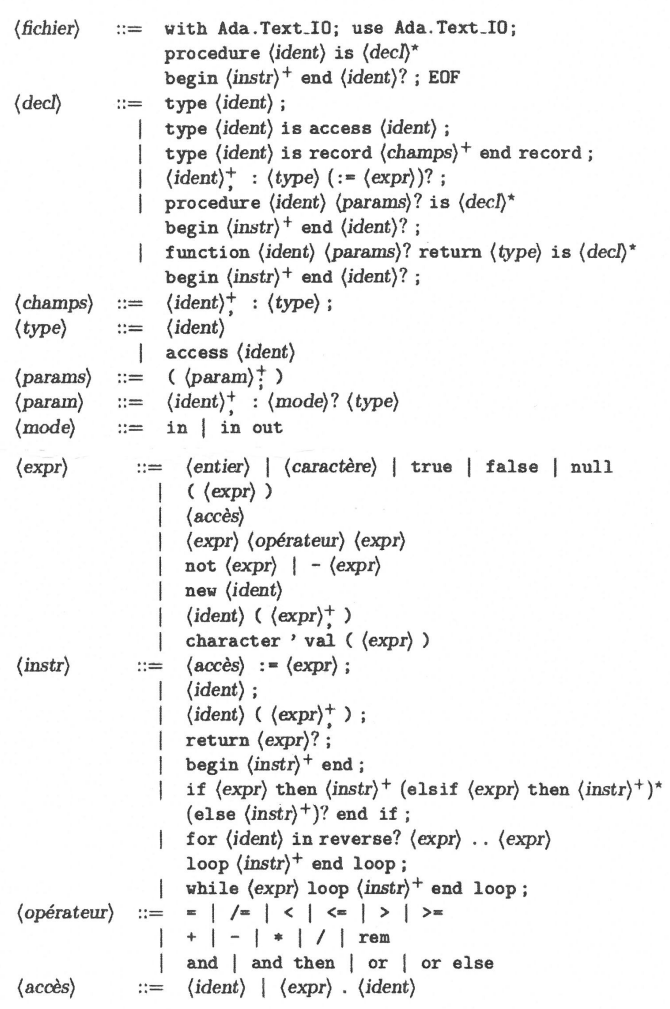
\includegraphics[width=0.8\textwidth]{grammaire_init}
        \caption{Grammaire initiale du Sujet}\label{fig:figure}
    \end{figure}

    \subsection{Étapes de transformation de la Grammaire}\label{subsec:etapes-de-transformation-de-la-grammaire}

    \subsubection{Grammaire originale en BNF}\label{subsec:grammaire-originale-en-bnf}

    La grammaire initiale du langage \textit{canAda}, avant sa transformation en grammaire LL(1), se présente comme suit en BNF sans les regex:

    \begin{lstlisting}[label={lst:lstlisting}]
        fichier -> $withAda.Text$_$IO$ $;$ $useAda.Text$_$IO$ $;$ $procedure$ $ident$ $is$ <decls> $begin$ <instrs> $end$ <hasident> $;$ $EOF$

        decl -> $type$ $ident$ $;$
               | $type$ $ident$ $is$ $access$ $ident$ $;$
               | $type$ $ident$ $is$ $record$ <champs> $end$ $record$ $;$
               | <identsep> $:$ <type> <typexpr> $;$
               | $procedure$ $ident$ <hasparams> $is$ <decls> $begin$ <instrs> $end$ <hasident> $;$
               | $function$ $ident$ <hasparams> $return$ <type> $is$ <decls> $begin$ <instrs> $end$ <hasident> $;$

        decls -> <decl> <decls>
                | $\epsilon$

        hasident -> $ident$
                   | $\epsilon$

        identsep -> $ident$ $,$ <identsep>
                   | ident

        champ -> <identsep> $:$ <type> $;$

        champs -> <champ> <champs>
                 | <champ>

        type -> $ident$
               | $access$ ident

        params -> $($ <paramsep> $)$

        hasparams -> <params>
                    | $\epsilon$

        paramsep -> <param> $;$ <paramsep>
                   | <param>

        typexpr -> $:=$ <expr>
                  | $\epsilon$

        param -> <identsep> $:$ <mode> <type>

        mode -> $in$
               | $in$ $out$
               | $\epsilon$

        expr -> $entier$
               | $caractère$
               | $true$
               | $false$
               | $null$
               | $($ <expr> $)$
               | <acces>
               | <expr> <opérateur> <expr>
               | $not$ <expr>
               | $-$ <expr>
               | $new$ $ident$
               | $ident$ ( <exprsep> )
               | $character$ $'$ $val$ $($ <expr> $)$

        exprsep -> <expr> $,$ <exprsep>
                  | <expr>

        hasexpr -> <expr>
                  | $\epsilon$

        instr -> <acces> $:=$ <expr> ;
                 | $ident$ $;$
                 | $ident$ ( <exprsep> ) $;$
                 | $return$ <hasexpr> $;$
                 | $begin$ <instrs> $end$ $;$
                 | $if$ <expr> $then$ <instrs> <elsif> <else> $end$ $if$ $;$
                 | $for$ $ident$ $in$ <hasreverse> <expr> .. <expr> $loop$ <instrs> $end$ $loop$ $;$
                 | $while$ <expr> $loop$ <instrs> $end$ $loop$ $;$

        elsif -> $elsif$ <expr> $then$ <instrs> <elsif>
                 | $\epsilon$

        else -> $else$ <instrs>
                 | $\epsilon$

        hasreverse -> $reverse$
                      | $\epsilon$

        instrs -> <instr> <instrs>
                  | <instr>

        opérateur -> $=$ | $/=$ | $<$ | $<=$ | $>$ | $>=$ | $+$ | $-$ | $*$ | $/$ | $rem$ | $and$ | $and$ $then$ | $or$ | $or$ $else$

        acces -> $ident$
                | <expr> $.$ $ident$

    \end{lstlisting}

    \subsubsection{Élimination de la Récursivité à Gauche}
    La grammaire initiale comportait plusieurs instances de récursivité à gauche.
    Par exemple, la règle:
    \begin{lstlisting}[label={lst:lstlisting2}]
        expr -> <accès>
        acces -> $ident$ | <expr> . ident
    \end{lstlisting}
    a été transformée en:
    \begin{lstlisting}[label={lst:lstlisting3}]
        expr -> $ident$ <primary2>
        primary2 -> $($ <exprsep> $)$ <acces> | <acces>
        acces -> $.$ ident <acces> | $\epsilon$
    \end{lstlisting}
    Cette modification élimine la (double ici) récursivité à gauche, rendant la grammaire adaptée pour une analyse LL(1).
    Une autre récursivité à gauche a été supprimé mais elle a été faite aussi à travers la priorisation des règles.

    \subsubsection{Factorisation à Gauche}
    La factorisation à gauche a été nécessaire pour certaines règles.
    Par exemple:
    \begin{lstlisting}[label={lst:lstlisting4}]
        exprsep -> <expr> $,$ <exprsep>
        exprsep -> <expr>
    \end{lstlisting}
    a été réécrite en:
    \begin{lstlisting}[label={lst:lstlisting5}]
        exprsep -> <expr> <exprsep$'$>
        exprsep$'$ -> $,$ <expr> <exprsep$'$> | $\epsilon$
    \end{lstlisting}
    Ceci assure que la règle peut être analysée de manière déterministe en LL(1).

    \subsubsection{Gestion des Priorités de Calculs}
    Pour gérer correctement les priorités des opérations, la grammaire a été ajustée.
    Par exemple, les opérations de multiplication et division ont été séparées des opérations d'addition et de soustraction pour respecter leur priorité:
    \begin{lstlisting}[label={lst:lstlisting6}]
        expr -> <expr> <operateur> <expr>
    \end{lstlisting}
    a été réécrite en:
    \begin{lstlisting}[label={lst:lstlisting7}]
        expr -> <or_expr>
        or_expr -> <and_expr> <or_expr$'$>
        or_expr$'$ -> $or$ <or_expr$'$2> | $\epsilon$
        or_expr$'$2 -> <and_expr> <or_expr$'$>
        or_expr$'$2 -> $else$ <and_expr> <or_expr$'$>
        and_expr -> <not_expr> <and_expr$'$>
    \end{lstlisting}
    [\dots]
    \begin{lstlisting}[label={lst:lstlisting8}]
        unary_expr -> $-$ <unary_expr>
        unary_expr -> <primary>
        primary -> $entier$
        primary -> $caractère$
        primary -> $true$
        primary -> $false$
        primary -> $null$
        primary -> $($ <expr> $)$
        primary -> $ident$ <primary2>
        primary -> $new$ $ident$
        primary -> $character$ $'$ $val$ ( <expr> )
    \end{lstlisting}
    Cela permet de respecter la hiérarchie des opérations dans les expressions arithmétiques.

    Les ensembles de sélection distincts ont été calculés pour assurer une sélection univoque lors de l'analyse.

    Ces étapes illustrent comment la grammaire initiale a été transformée en une grammaire LL(1), adaptée pour une analyse syntaxique efficace et précise du langage \textit{canAda}

    \subsection{Grammaire Transformée en LL(1)}\label{subsec:grammaire-transformee-en-ll(1)}
    La grammaire transformée en LL(1) se présente comme suit:
    \begin{lstlisting}[label={lst:lstlisting9}]
        fichier -> $withAda.Text$_$IO$ $;$ $useAda.Text$_$IO$ $;$ $procedure$ $ident$ $is$ decls $begin$ instrs $end$ hasident $;$ $EOF$
        decl -> $type$ $ident$ hasischoose $;$
        decl -> identsep $:$ type_n typexpr $;$
        decl -> $procedure$ ident hasparams $is$ decls $begin$ instrs $end$ hasident $;$
        decl -> $function$ $ident$ hasparams $return$ type_n $is$ decls $begin$ instrs $end$ hasident $;$

        hasischoose -> $is$ accorrec | $\epsilon$

        accorrec -> $access$ $ident$
        accorrec -> $record$ champs $end$ $record$

        decls -> decl decls
        decls -> $\epsilon$

        hasident -> $ident$
        hasident -> $\epsilon$

        identsep -> $ident$ identsep2

        identsep2 -> $,$ identsep
        identsep2 -> $\epsilon$

        champ -> identsep $:$ type_n $;$

        champs -> champ champs2

        champs2 -> champs | $\epsilon$

        type_n -> $ident$
        type_n -> $access$ $ident$

        params -> $($ paramsep $)$

        hasparams -> params
        hasparams -> $\epsilon$

        paramsep -> param paramsep2

        paramsep2 -> $;$ paramsep
        paramsep2 -> $\epsilon$

        typexpr -> $:=$ expr
        typexpr -> $\epsilon$

        param -> identsep $:$ mode type_n

        mode -> $in$ modeout
        mode -> $\epsilon$

        modeout -> $out$
        modeout -> $\epsilon$

        expr -> or_expr

        or_expr -> and_expr or_expr$'$

        or_expr$'$ -> $or$ or_expr$'$2
        or_expr$'$ -> $\epsilon$

        or_expr$'$2 -> and_expr or_expr$'$
        or_expr$'$2 -> $else$ and_expr or_expr$'$

        and_expr -> not_expr and_expr$'$

        and_expr$'$ -> $and$ and_expr$'$2
        and_expr$'$ -> $\epsilon$

        and_expr$'$2 -> not_expr and_expr$'$
        and_expr$'$2 -> $then$ not_expr and_expr$'$

        not_expr -> equality_expr not_expr$'$

        not_expr$'$ -> $not$ equality_expr not_expr$'$
        not_expr$'$ -> $\epsilon$

        equality_expr -> relational_expr equality_expr$'$

        equality_expr$'$ -> $=$ relational_expr equality_expr$'$
        equality_expr$'$ -> $/=$ relational_expr equality_expr$'$
        equality_expr$'$ -> $\epsilon$

        relational_expr -> additive_expr relational_expr$'$

        relational_expr$'$ -> $<$ additive_expr relational_expr$'$
        relational_expr$'$ -> $<=$ additive_expr relational_expr$'$
        relational_expr$'$ -> $>$ additive_expr relational_expr$'$
        relational_expr$'$ -> $>=$ additive_expr relational_expr$'$
        relational_expr$'$ -> $\epsilon$

        additive_expr -> multiplicative_expr additive_expr$'$

        additive_expr$'$ -> $+$ multiplicative_expr additive_expr$'$
        additive_expr$'$ -> $-$ multiplicative_expr additive_expr$'$
        additive_expr$'$ -> $\epsilon$

        multiplicative_expr -> unary_expr multiplicative_expr$'$

        multiplicative_expr$'$ -> $*$ unary_expr multiplicative_expr$'$
        multiplicative_expr$'$ -> $/$ unary_expr multiplicative_expr$'$
        multiplicative_expr$'$ -> $rem$ unary_expr multiplicative_expr$'$
        multiplicative_expr$'$ -> $\epsilon$

        unary_expr -> $-$ unary_expr
        unary_expr -> primary

        primary -> $entier$
        primary -> $caractère$
        primary -> $true$
        primary -> $false$
        primary -> $null$
        primary -> $($ expr $)$
        primary -> $ident$ primary2
        primary -> $new$ $ident$
        primary -> $character$ $'$ $val$ $($ expr $)$

        primary2 -> $($ exprsep $)$ acces
        primary2 -> acces

        exprsep -> expr exprsep2

        exprsep2 -> $,$ exprsep
        exprsep2 -> $\epsilon$

        hasexpr -> expr
        hasexpr -> $\epsilon$

        instr -> $ident$ instr2
        instr -> $return$ hasexpr $;$
        instr -> $begin$ instrs $end$ $;$
        instr -> $if$ expr $then$ instrs elifn elsen $end$ $if$ $;$
        instr -> $for$ ident $in$ hasreverse expr $..$ expr $loop$ instrs $end$ $loop$ $;$
        instr -> $while$ expr $loop$ instrs $end$ $loop$ $;$

        instr2 -> instr3 $:=$ expr $;$
        instr2 -> $($ exprsep $)$ instr3 hasassign $;$
        instr2 -> $;$

        instr3 -> $.$ $ident$ instr3
        instr3 -> $\epsilon$

        hasassign -> $:=$ expr
        hasassign -> $\epsilon$

        elifn -> $elif$ expr $then$ instrs elifn
        elifn -> $\epsilon$

        elsen -> $else$ instrs
        elsen -> $\epsilon$

        hasreverse -> $reverse$
        hasreverse -> $\epsilon$

        instrs -> instr instrs2

        instrs2 -> instr instrs2
        instrs2 -> $\epsilon$

        acces -> $.$ $ident$ acces
        acces -> $\epsilon$
    \end{lstlisting}

    \subsection{Table LL(1)}\label{subsec:table-ll(1)}

    A l'aide de la grammaire transformée en LL(1), nous avons pu construire la table LL(1) suivante pour produire notre Parser.
    Ci-dessous, nous présentons une partie de la table LL(1) pour des raisons de lisibilité.

    \begin{figure}[H]
        \centering
        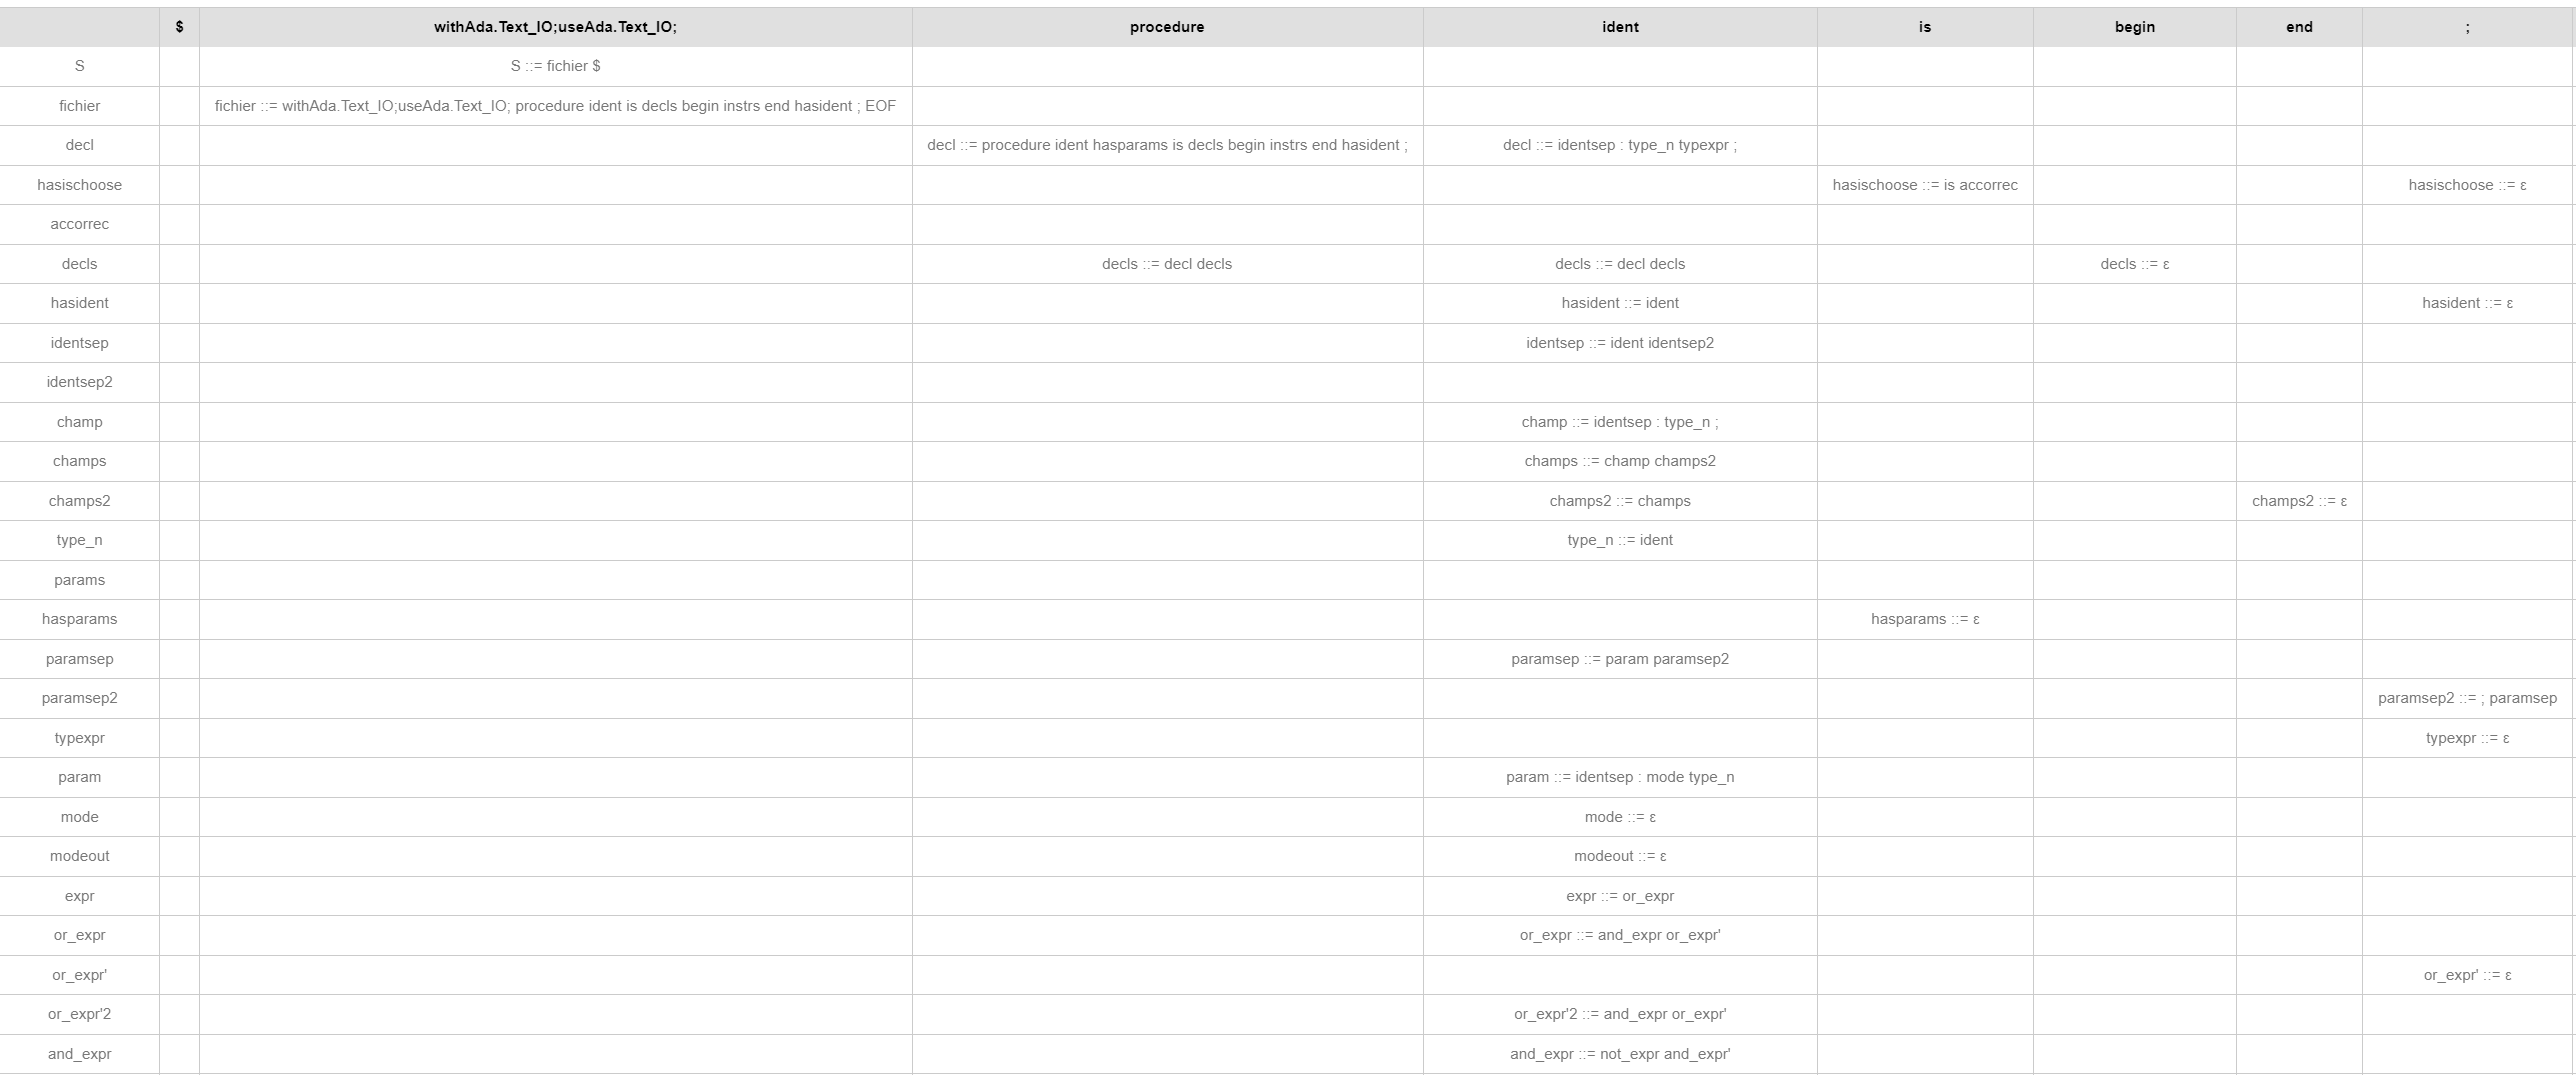
\includegraphics[width=1\textwidth]{partial_table}
        \caption{Table partielle LL(1)}\label{fig:figure2}
    \end{figure}

    \section{Analyse Lexicale pour canAda}\label{sec:analyse-lexicale-pour-canada}

    L'analyse lexicale, une étape cruciale dans le processus de compilation, est gérée par notre classe \textit{Lexer}.
    Cette classe est responsable de la conversion du code source en une série de tokens, facilitant ainsi l'analyse syntaxique ultérieure.
    Elle contient un \textit{PeekingReader} codé par nos soins, qui permet de lire dans le flux de caractères pour identifier correctement les tokens complexes tout en conservant ce qui a été lu et en lisant caractère par caractère.
    Elle contient également un \textit{ErrorService} qui permet de gérer les erreurs lexicales mais aussi une map de mots clés qui permet de gérer les mots clés du langage, les opérateurs et les symboles.

    \subsection{Structure et Fonctionnement du Lexer}\label{subsec:structure-et-fonctionnement-du-lexer}

    La classe \textit{Lexer} lit le code source et identifie les différents tokens en se basant sur un ensemble de règles prédéfinies, il est codé à l'aide du pattern \textit{Singleton} pour éviter d'avoir plusieurs instances de la classe.
    Chaque token est une instance de la classe \textit{Token}, qui contient des informations telles que le type de token et la valeur lexicale associée contenu dans l'enum \textit{Tag}.

    \subsection{Gestion des Tokens}\label{subsec:gestion-des-tokens}

    Des classes spécifiques, comme \textit{Tag} et \textit{PeekingReader}, sont utilisées pour catégoriser les tokens et gérer efficacement la lecture en avance du code source.
    La classe \textit{Tag} définit les différents types de tokens, c'est une enum, tandis que \textit{PeekingReader} permet de lire en avance dans le flux de caractères pour identifier correctement les tokens complexes en se passant donc d'un automate à états finis.
    Cela repose sur deux fonctions complexes qui permettent de lire le flux de caractères et de déterminer si le caractère courant est la fin d'un token.

    \begin{lstlisting}[label={lst:lstlisting1}]
        /**
         * Check if the current character is the end of a token
         *
         * @return true if the current character is the end of a token, false otherwise
         */
        private boolean isEndOfToken() {
            char current = (char) currentChar;
            int nextInt = this.reader.peek(1);
            char next = (char) nextInt;

            boolean isCurrentLetterOrDigit = Character.isLetterOrDigit(current) || current == '_';
            boolean isNextLetterOrDigit = Character.isLetterOrDigit(next) || next == '_';
            boolean isNextWhitespace = Character.isWhitespace(next);

            // If the current character is a whitespace or the end of the file, the current character is the end of the token
            if (nextInt == -1 || isNextWhitespace) {
                return true;
            }
            // If the current character is an identifier or an integer, the next character must not be a letter or a digit
            if (isCurrentLetterOrDigit) {
                return !isNextLetterOrDigit;
            }

            Token token = this.matchToken(lexeme.toString());

            // If the current character is a token and the next character is not a token, the current character is the end of the token
            if (token.tag() != Tag.UNKNOWN) {
                Token nextToken = this.matchToken(lexeme.toString() + next);
                return nextToken.tag() == Tag.UNKNOWN;
            }

            return false;
        }
    \end{lstlisting}

    \begin{lstlisting}[label={lst:lstlisting12}]
        public Token nextToken() {

            while ((this.currentChar = this.reader.read()) != -1) {

                if (this.isComment()) {
                    this.skipComment();
                } else if (Character.isWhitespace((char) currentChar)) {
                    this.skipWhitespace();
                } else if (isCharacterLiteral()) {
                    return this.readCharacterLiteral();
                } else {
                    lexeme.append((char) currentChar);
                    if (this.isEndOfToken()) {
                        Token token = this.matchToken(lexeme.toString());
                        lexeme.setLength(0); // clear the StringBuilder
                        if (token.tag() == Tag.UNKNOWN) {
                            this.errorService.registerLexicalError(new UnknownTokenException(token));
                        }
                        return token;
                    }
                }
            }

            this.reader.close();
            return new Token(Tag.EOF, this.reader.getCurrentLine(), lexeme.toString());
        }
    \end{lstlisting}

    \subsection{Optimisation et Fiabilité}\label{subsec:optimisation-et-fiabilite}

    Le \textit{Lexer} est conçu pour être à la fois rapide et fiable, capable d'identifier précisément les tokens même dans des cas de syntaxe complexe grâce aux fonctions présentées ci-dessus.
    Cette précision est essentielle pour garantir une analyse syntaxique sans erreur dans les étapes suivantes du processus de compilation.

    \section{Analyse Syntaxique}\label{sec:analyse-syntaxique}

    \subsection{Structure et Fonctionnement}\label{subsec:structure-et-fonctionnement}

    La classe \textit{Parser} a été conçue pour analyser les programmes écrits dans le langage \textit{canAda}, il est codé, lui aussi, à l'aide du pattern \textit{Singleton} pour éviter d'avoir plusieurs instances de la classe.
    Il contient le token courant et l'analyseur lexical, qui sont utilisés pour analyser le programme source.
    Chaque méthode de cette classe correspond à un non-terminal de la grammaire LL(1) et est responsable de l'analyse d'une structure syntaxique spécifique du langage.
    Par exemple, une méthode \textit{expr()} est utilisée pour analyser les expressions, correspondant au non-terminal \textit{expr} de la grammaire.
    Ces méthodes sont appelées récursivement pour construire l'arbre syntaxique du programme source.

    \begin{lstlisting}[label={lst:lstlisting10}]
        @PrintMethodName
        private void expr() {
            switch (this.currentToken.tag()) {
                case IDENT, OPEN_PAREN, DOT, ENTIER, CARACTERE, TRUE, FALSE, NULL, NEW, CHARACTER -> {
                    or_expr();
                }
            }
        }
    \end{lstlisting}


    \subsection{Interaction avec l'Analyseur Lexical}\label{subsec:interaction-avec-l'analyseur-lexical}

    Le \textit{Parser} interagit étroitement avec l'analyseur lexical, recevant un flux de tokens qui sont analysés selon les règles de la grammaire.
    Cette interaction est cruciale pour la décomposition correcte du programme source en ses composants syntaxiques.
    On lit les tokens un par un et on les compare avec les règles de la grammaire.
    Si le token correspond à la règle, on passe au token suivant.
    Si le token ne correspond pas à la règle, on génère une erreur syntaxique.

    \begin{lstlisting}[label={lst:lstlisting11}]
        @PrintMethodName
        private void analyseTerminal(Tag tag) {
            System.out.println("\t\t↪️ " + this.currentToken);
            if (!(this.currentToken.tag() == tag)) {
                Token expectedToken = new Token(tag, this.currentToken.line(), TagHelper.getTagString(tag));
                if (expectedToken.tag() == Tag.SEMICOLON) {
                    this.errorService.registerSyntaxWarning(new MissingSemicolonException(this.currentToken));
                } else {
                this.errorService.registerSyntaxError(new UnexpectedTokenException(expectedToken, this.currentToken));}
            }
            // Contient le prochain token ou <EOF, currentLine,""> si fin de fichier
            if (this.currentToken.tag() == Tag.EOF) {
                return;
            }
            this.currentToken = lexer.nextToken();
        }
    \end{lstlisting}

    \subsection{Gestion des Erreurs Syntaxiques}\label{subsec:gestion-des-erreurs-syntaxiques}

    Un aspect essentiel du \textit{Parser} est sa capacité à gérer les erreurs syntaxiques comme nous le voyons dans le code ci-dessus.
    Lorsque le programme source ne respecte pas les règles de la grammaire, des messages d'erreur descriptifs sont générés, indiquant la ligne et le token attendu par rapport au token reçu, facilitant la localisation et la correction des erreurs par les développeurs.
    On a notamment appliqué le \textit{Panic Mode} pour gérer les erreurs syntaxiques.
    Le \textit{Parser} continue à analyser le programme source jusqu'à la fin tout en indiquant les erreurs rencontrées.

    \section{Construction de l'Arbre Abstrait Syntaxique pour canAda}\label{sec:construction-de-l'arbre-abstrait-syntaxique-pour-canada}

    La construction de l'arbre abstrait syntaxique (AST) est une étape essentielle du processus de compilation du langage \textit{canAda}.
    L'AST représente la structure syntaxique du programme source d'une manière qui est à la fois concise et facile à manipuler pour les étapes suivantes de la compilation.

    \subsection{Structure et Fonctionnement de l'AST}\label{subsec:structure-et-fonctionnement-de-l'ast}

    Notre système d'AST est construit autour de la classe \textit{ASTNode}, qui sert de classe de base pour les différents types de nœuds de l'arbre.
    Chaque nœud spécifique, comme \textit{OperatorNode}, \textit{ParameterNode}, ou \textit{ProgramNode}, hérite de \textit{ASTNode} et représente une construction syntaxique spécifique du langage.

    Par exemple, \textit{OperatorNode} représente une opération arithmétique ou logique, tandis que \textit{ProgramNode} représente la structure globale du programme \textit{canAda}.

    \begin{lstlisting}[label={lst:lstlisting13}]
        public class ProgramNode extends ASTNode {
            private ProcedureDeclarationNode rootProcedure;

            public void setRootProcedure(ProcedureDeclarationNode rootProcedure) {
                this.rootProcedure = rootProcedure;
                rootProcedure.setParent(this);
            }

        }
    \end{lstlisting}

    \begin{lstlisting}[label={lst:lstlisting15}]
        public class OperatorNode extends ASTNode {
            private String operator;

            public OperatorNode(String operator) {
                this.operator = operator;
            }

        }
    \end{lstlisting}

    Et ainsi de suite pour chaque nœud de l'arbre.
    On utilise alors notre fonction \textit{Override} \textit{toString()} pour afficher l'arbre abstrait syntaxique de manière recursive qui est dans notre classe abstraite qui extend de nos différents nœuds.
    Ainsi on a juste a appeler la fonction \textit{toString()} sur le nœud racine de l'arbre pour afficher l'arbre abstrait syntaxique qui récupère les différents nœuds de l'arbre et les affiche de manière récursivee en recupérant les différents attributs de chaque nœud.

    \begin{lstlisting}[label={lst:lstlisting14}]
        public String toString() {
            Field[] fields = this.getClass().getDeclaredFields();
            String className = this.getClass().getSimpleName();
            StringBuilder res = new StringBuilder(colorize(className, Attribute.YELLOW_TEXT()) + " : { \n");
            if (isJson) {
                res = new StringBuilder("{ \n");
            }
            int lastIndex = fields.length - 1;

            for (int i = 0; i < fields.length; i++) {
                Field field = fields[i];
                field.setAccessible(true);
                try {
                    Object attributeValue = field.get(this);
                    if (attributeValue instanceof String) {
                        attributeValue = colorize("\"" + attributeValue + "\"", Attribute.GREEN_TEXT());
                    }
                    if (attributeValue == null) {
                        attributeValue = colorize("null", Attribute.BRIGHT_MAGENTA_TEXT());
                    }
                    res.append("\t").append("\"").append(colorize(field.getName(), Attribute.RED_TEXT())).append("\"").append(" : ").append(attributeValue);
                    if (i < lastIndex || !isJson) {
                        res.append(",");
                    }
                    res.append(" \n");

                } catch (IllegalAccessException e) {
                    System.err.println("Erreur lors de l'acces au champ " + field.getName());
                }
            }
            res.append("}");
            return format(res.toString());
        }
    \end{lstlisting}

    \subsection{Représentation des Structures Syntaxiques}\label{subsec:representation-des-structures-syntaxiques}

    Les nœuds de l'AST capturent les éléments essentiels des structures syntaxiques du programme, comme les opérations, les paramètres, et la structure globale du programme.
    Par exemple, \textit{OperatorNode} représente une opération arithmétique ou logique, tandis que \textit{ProgramNode} représente la structure globale du programme \textit{canAda}.

    \subsection{Rôle dans le Processus de Compilation}\label{subsec:role-dans-le-processus-de-compilation}

    L'AST joue un rôle central dans le processus de compilation.
    Après l'analyse syntaxique, le programme source est transformé en un AST, qui est ensuite utilisé pour les étapes de vérification sémantique, d'optimisation, et de génération de code.
    Cette représentation permet une manipulation plus aisée et plus efficace du programme source.

    \section{Tests et Validation}\label{sec:tests-et-validation}

    \subsection{Pour un code source valide}\label{subsec:pour-un-code-source-valide}

    Voici un code source valide en canAda qui permet de tester notre compilateur :

    \begin{lstlisting}[label={lst:lstlisting16}]
        with Ada.Text_IO; useAda.Text_IO;
        procedure Main is
            A : Integer := 5;
            B : Integer := 10;
            Sum : Integer;
        begin
            Sum := A + B;
        end Main;
    \end{lstlisting}

    On obtient alors après l'analyse lexicale et syntaxique la sortie suivante, on l'a découpé en 3 parties pour plus de lisibilité et laisser sur fond noir pour faciliter la lisibilité des couleurs :

    \begin{figure}[H]
        \centering
        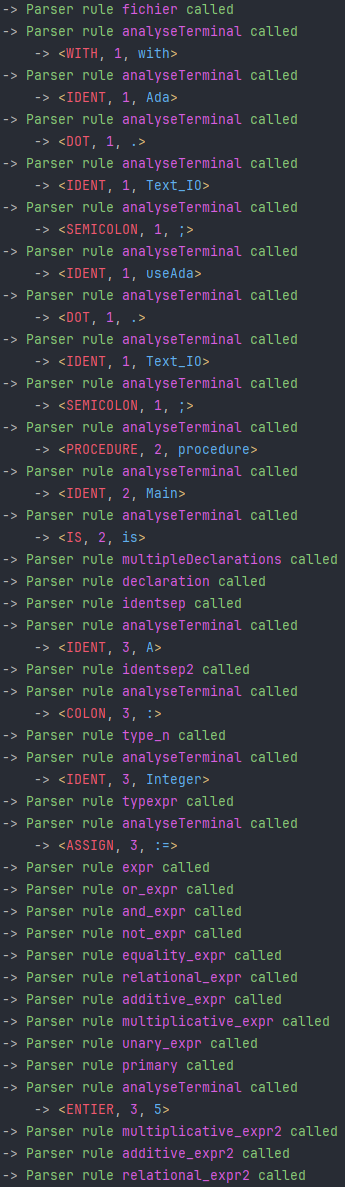
\includegraphics[width=0.3\textwidth]{sortie1}
        \hfill
        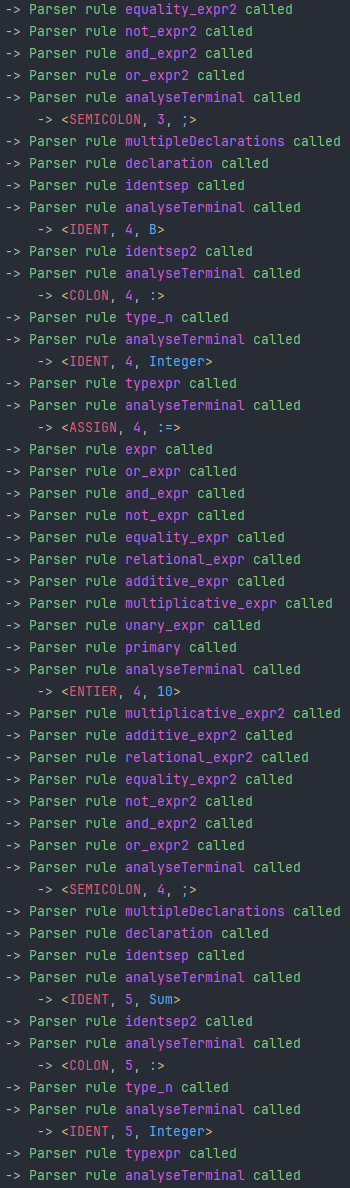
\includegraphics[width=0.3\textwidth]{sortie2}
        \hfill
        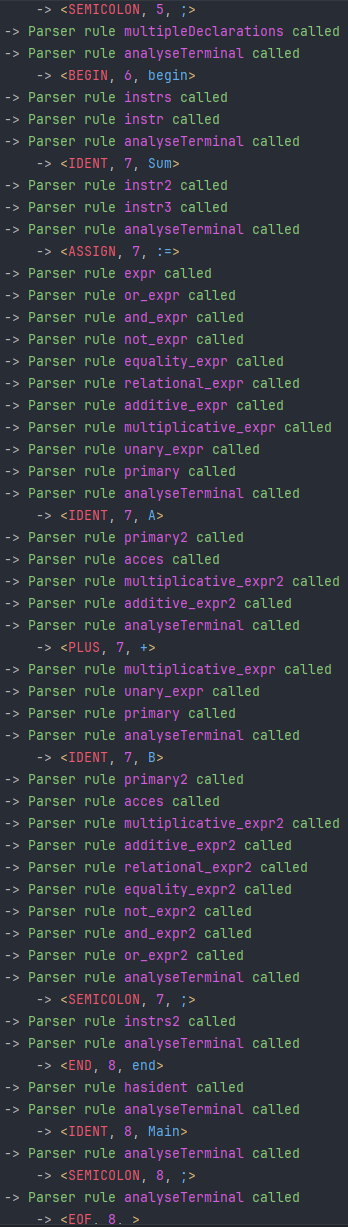
\includegraphics[width=0.3\textwidth]{sortie3}
        \caption{Sortie découpée de gauche à droite}\label{fig:figure4}
    \end{figure}

    Et on obtient l'arbre abstrait suivant en sortie et donc ici en json :

    \begin{figure}[H]
        \centering
        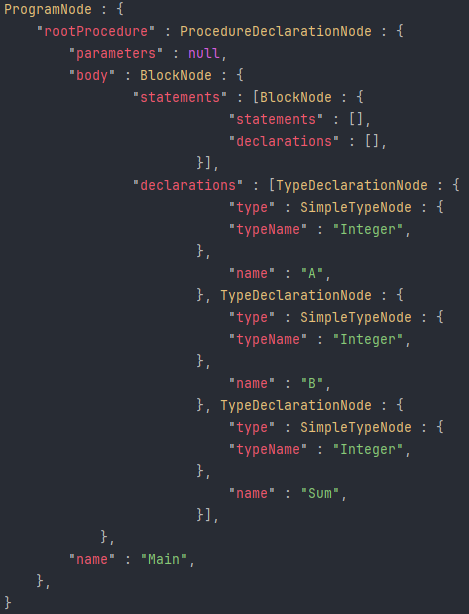
\includegraphics[width=1\textwidth]{arbre_json}
        \caption{Arbre abstrait}\label{fig:figure5}
    \end{figure}

    Et à l'aide de notre script python et de graphviz on obtient l'arbre abstrait suivant :

    \begin{figure}[H]
        \centering
        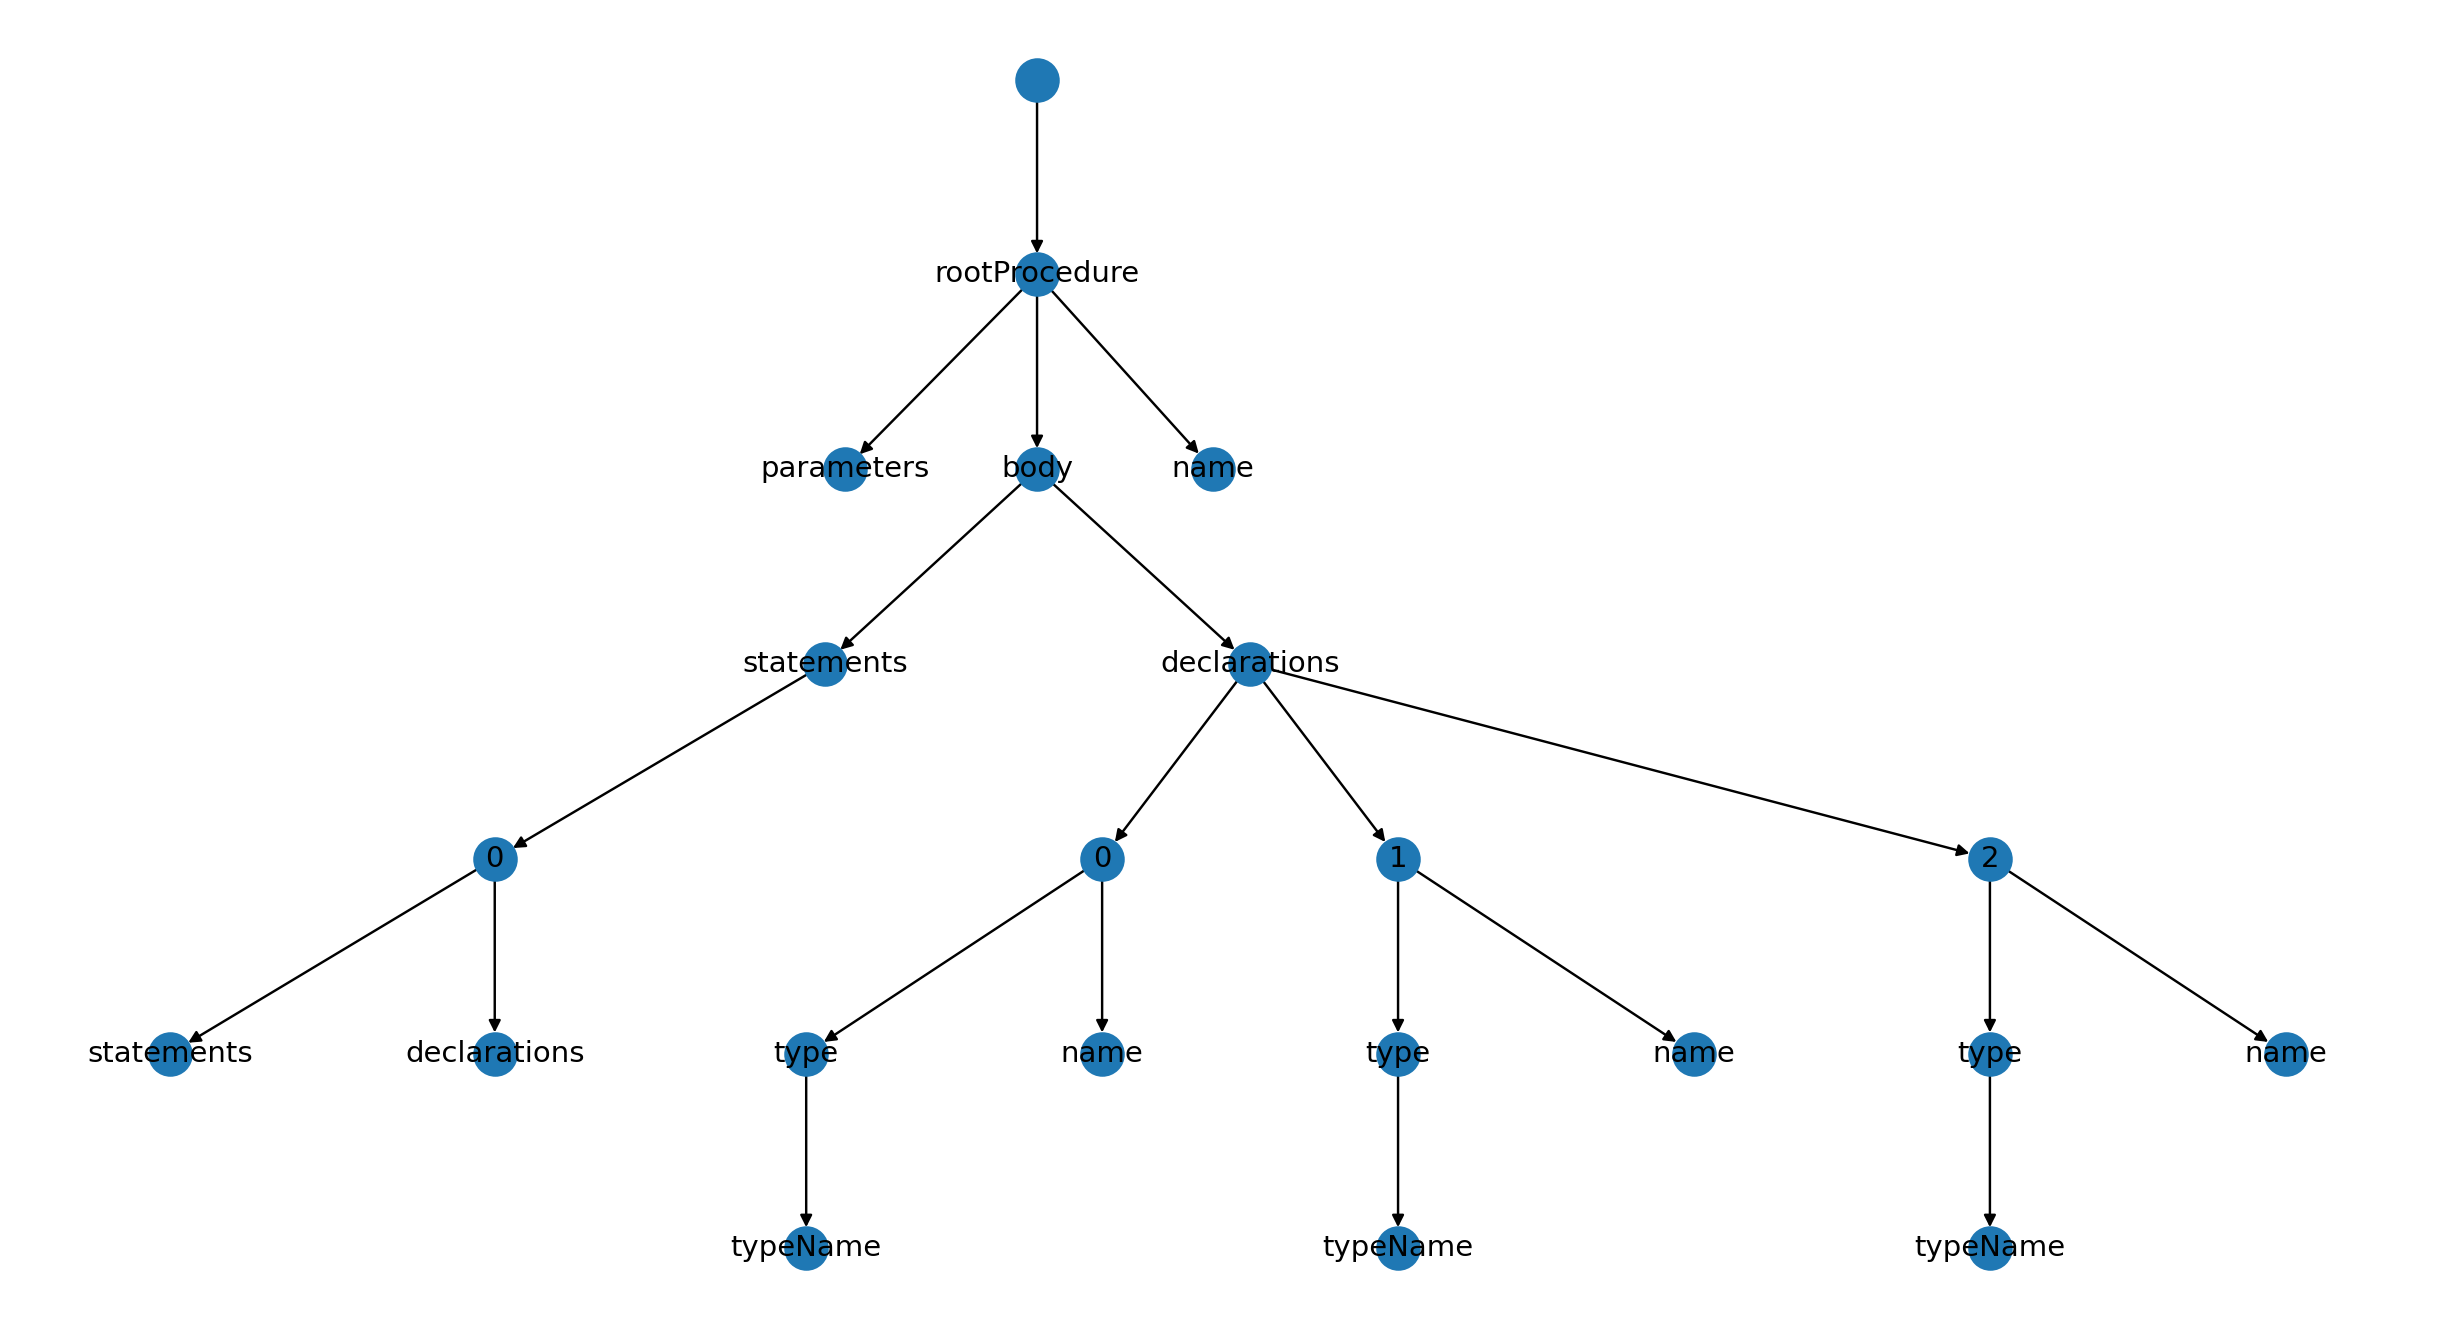
\includegraphics[width=1\textwidth]{arbre_draw}
        \caption{Arbre abstrait}\label{fig:figure6}
    \end{figure}

    \subsection{Pour un code source invalide}\label{subsec:pour-un-code-source-invalide}

    Voici un code source invalide en canAda qui permet de tester notre compilateur, on a volontairement rajouter un ; en trop à la fin de la ligne 5 :

    \begin{lstlisting}[label={lst:lstlisting17}]
        with Ada.Text_IO; useAda.Text_IO;
        procedure Main is
            A : Integer := 5;
            B : Integer := 10;
            Sum : Integer;
        begin ;
            Sum := A + B;
        end Main;
    \end{lstlisting}

    On obtient alors après l'analyse lexicale et syntaxique la sortie suivante, on l'a découpé en 3 parties pour plus de lisibilité et laisser sur fond noir pour faciliter la lisibilité des couleurs :

    \begin{figure}[H]
        \centering
        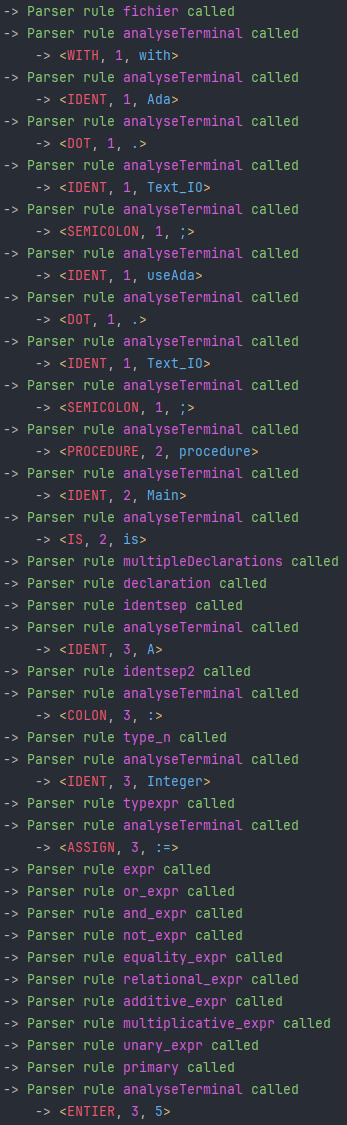
\includegraphics[width=0.3\textwidth]{sortie1_err}
        \hfill
        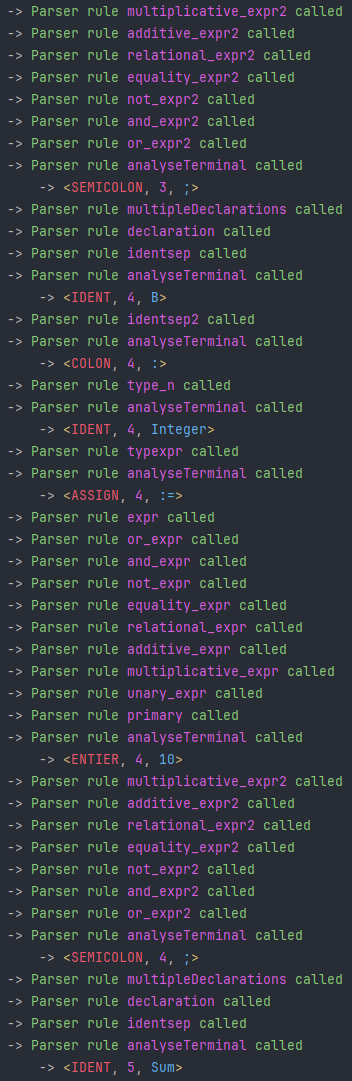
\includegraphics[width=0.3\textwidth]{sortie2_err}
        \hfill
        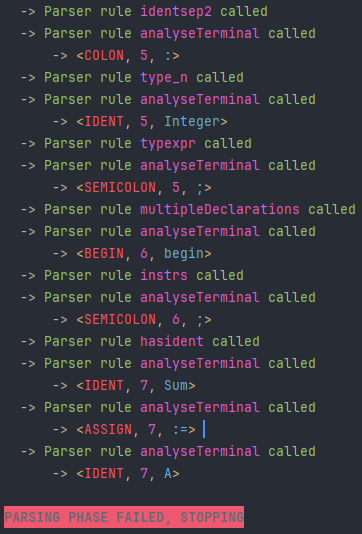
\includegraphics[width=0.3\textwidth]{sortie3_err}
        \caption{Sortie découpée de gauche à droite}\label{fig:figure7}
    \end{figure}

    Et on obtient les erreurs et les warnings suivantes :

    \begin{figure}[H]
        \centering
        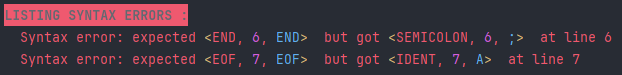
\includegraphics[width=1\textwidth]{syntax_err}
        \caption{Erreurs}\label{fig:figure8}
    \end{figure}

    \begin{figure}[H]
        \centering
        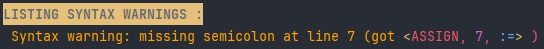
\includegraphics[width=1\textwidth]{syntax_warn}
        \caption{Warnings}\label{fig:figure9}
    \end{figure}

    On peut ainsi voir que notre compilateur est capable de gérer les erreurs syntaxiques et de les afficher de manière claire et précise.
    Ainsi que de nous aider à le corriger notamment à travers les warnings et le \textit{Panic Mode} qui permet de continuer à analyser le programme source jusqu'à la fin tout en indiquant les erreurs rencontrées.

    Ce qui conclue la partie sur les tests et la validation de notre compilateur.
    Bien évidemment, de nombreux autres tests ont été réalisés pour valider notre compilateur notamment des tests unitaires pour tester le \textit{Lexer} et le \textit{Parser} ainsi que la construction l'arbre asbtrait.

    \section{Gestion de projet}\label{sec:gestion-de-projet}

    \subsection{Équipe de projet}\label{subsec:equipe-de-projet}
    Ce projet est un projet local réalisé en groupe de 3 personnes~:
    \begin{itemize}
        \item Alexis MARCEL
        \item Lucas LAURENT
        \item Noé STEINER
    \end{itemize}

    \subsection{Organisation au sein de l’équipe projet}\label{subsec:organisation-au-sein-de-lequipe-projet}
    Nous avons réalisé plusieurs réunions, en présentiel dans les locaux de Télécom Nancy mais la plupart de notre collaboration a eu lieu sur Discord.
    Ces réunions nous ont permis de mettre en commun nos avancées régulièrement, de partager nos connaissances sur des problématiques et de nous organiser de manière optimale.
    En plus des réunions d'avancement régulières, nous avons également réalisé des réunions techniques afin de résoudre un problème ou bien de réfléchir à la conception.

    Ensuite, nous avons utilisé GitLab pour gérer les différentes versions du développement de notre application, ainsi que les différentes
    branches nous permettant de travailler simultanément sans conflit.

    \subsection{Matrice RACI}\label{subsec:matrice-raci}
    Nous avons choisi de ne pas faire de matrice RACI à cause des choix d'organisation que nous avons faits.
    En effet, nous avons décidé de travailler en groupe sur toutes les tâches, ce qui fait que nous sommes tous responsables de toutes les tâches et qu'il n'y a, de ce fait,
    pas de répartition précise des tâches.

    \begin{figure}[H]
        \centering
        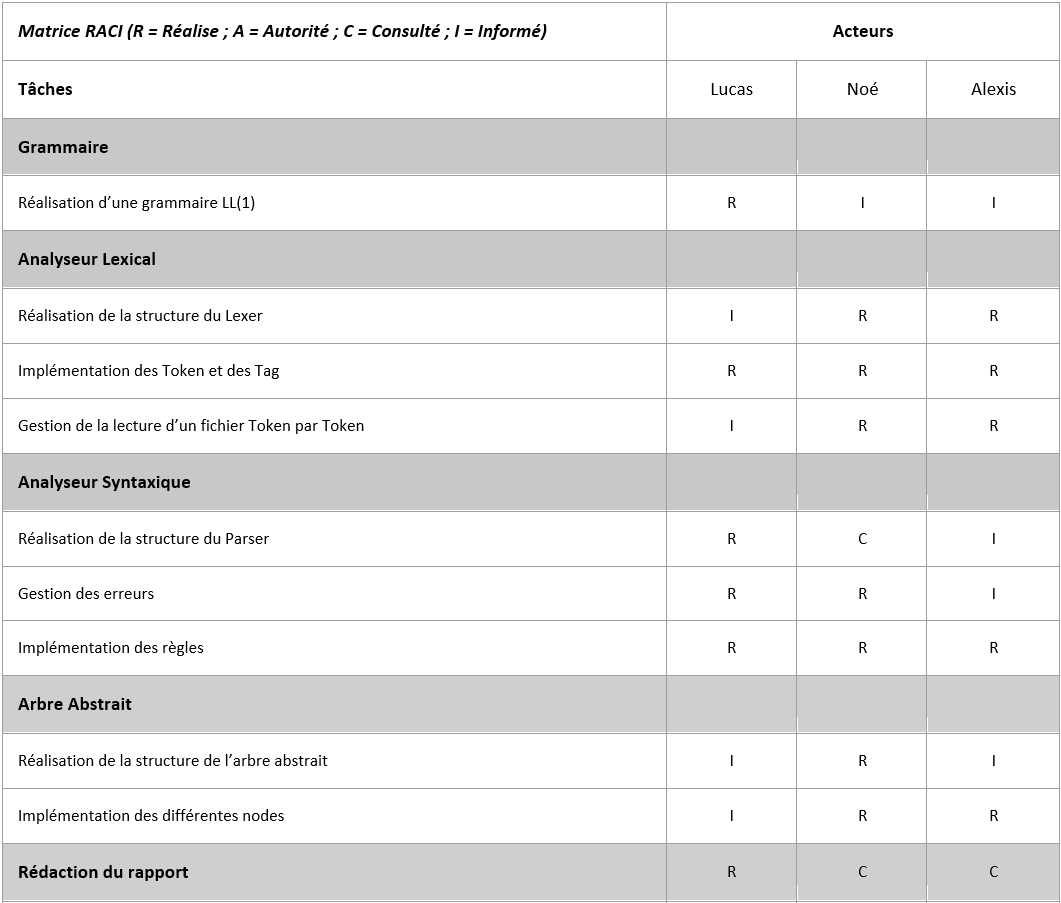
\includegraphics[width=1\textwidth]{RACI}
        \caption{Matrice RACI}\label{fig:figure3}
    \end{figure}

    \subsection{Répartition du Temps de Travail sur le Projet}\label{subsec:repartition-du-temps-de-travail-sur-le-projet}

    On peut voir que la répartition du temps de travail est équilibrée entre les membres de l'équipe, ce qui a permis une contribution égale de tous les membres de l'équipe :
    \newline

    \begin{tabular}{@{}llll@{}}
        \toprule
        Tâche & Lucas & Noé & Alexis \\ \midrule
        Grammaire & 10h & - & - \\
        Structure du Lexer & - & 2h & 4h \\
        Lecture du fichier (token par token) & - & 5h & 7h \\
        Implémentation des Token et des Tag & 2h & 2h & 2h \\
        Structure du Parser & 1h & - & - \\
        Gestion des erreurs & 4h & 4h & - \\
        Implémentation des règles & 3h & 3h & 3h \\
        Structure de l'arbre abstrait & - & 2h & - \\
        Implémentation des différents nodes & - & 6h & 6h \\
        Rédaction du rapport & 4h & - & - \\
        \midrule
        Total & 24h & 24h & 22h \\ \bottomrule
    \end{tabular}

    \section{Conclusion}\label{sec:conclusion}
    Ce rapport a présenté en détail le processus de développement d'un compilateur pour le langage \textit{canAda}, réalisé dans le cadre du module PCL1 à TELECOM Nancy.
    Le projet a débuté par la transformation de la grammaire originale en une grammaire LL(1), adaptée pour une analyse syntaxique précise.
    Cette transformation a impliqué l'élimination de la récursivité à gauche, la factorisation, et la gestion des priorités de calculs pour assurer une analyse déterministe.

    L'analyse lexicale a été effectuée par le \textit{Lexer}, un composant clé qui convertit le code source en tokens, en s'appuyant sur un ensemble de règles prédéfinies et un système efficace de lecture en avance et d'une astuce pour déterminer la fin d'un token ce qui nous a permis de nous passer d'un automate à états finis.
    La classe \textit{Parser}, quant à elle, a joué un rôle essentiel dans l'analyse syntaxique, en décomposant le programme source en ses composants syntaxiques, tout en gérant les erreurs syntaxiques de manière robuste.

    La construction de l'arbre abstrait syntaxique (AST) a été une étape cruciale, permettant une représentation concise et manipulable du programme source pour les étapes ultérieures de la compilation.
    Chaque nœud de l'AST, tel que \textit{OperatorNode} ou \textit{ProgramNode}, a capturé des éléments essentiels des structures syntaxiques du langage \textit{canAda}.

    La répartition du temps de travail sur les différentes tâches a été équilibrée, assurant ainsi une contribution égale de tous les membres de l'équipe.

    En conclusion, ce projet a non seulement abouti à la création d'un compilateur fonctionnel pour \textit{canAda} mais a également permis aux membres de l'équipe d'approfondir leurs compétences en informatique, notamment dans les domaines de l'analyse lexicale et syntaxique, ainsi que dans la construction et la manipulation d'arbres abstraits.
    Ce projet représente une étape significative dans notre parcours d'ingénieurs en informatique, nous préparant efficacement à des applications concrètes dans divers secteurs technologiques.

    Il a également renforcé notre compréhension des fondamentaux de la compilation, une compétence essentielle pour tout développeur de logiciels ainsi que pour tout ingénieur en informatique.

\end{document}
